\documentclass[a4paper, 12pt]{article}

%\usepackage{savetrees}
\usepackage{graphicx}
\usepackage{subfig}
\usepackage{longtable}

%code for creating python code snippets
\usepackage{float}
\floatstyle{ruled}
\newfloat{python}{thp}{lop}
\floatname{python}{Listing}
%end code for creating python code snippets

\graphicspath{{./images/}}
\title {Student Robotics 2009\\ Assembly Guide}
\date{\today}
\setcounter{tocdepth}{1}


\begin{document}

\maketitle

\noindent This document explains how to connect up the Student Robotics electronics kit. It is a \textit{Getting Started Guide} and is not a comprehensive description of the hardware. For more information about individual boards, see the respective documentation, available from the website: http://www.srobo.org 

\section{Before You Begin}

\section{Identify Kit Components}
Use the glossary in section \ref{sec:glossary} to identify the different components. This will make the following stages easier.

\newpage
%Glossary of components, terms

\section{Glossary}
\label{sec:glossary}
\begin{longtable}{| l | l| l |}
\hline
\textbf{Component} & \textbf{Description} & \textbf{Quantity} \\ \hline
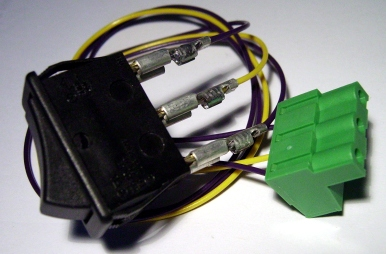
\includegraphics[height=2cm]{chrg-run-sw}  & Charge/Run switch & 1 \\ \hline
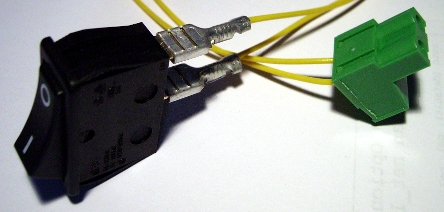
\includegraphics[height=2cm]{on-off-sw}  & On/Off Switch & 1 \\ \hline
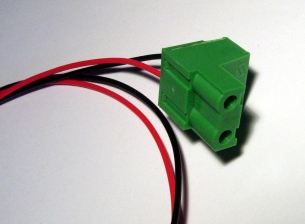
\includegraphics[height=2cm]{battery-con}  & Battery Connector & 1 \\ \hline
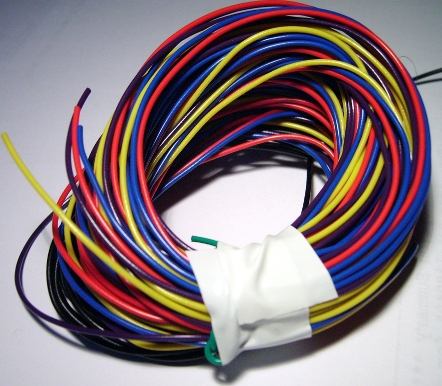
\includegraphics[height=2cm]{wire}  & Multi-core Electrical Wire & 5 \\ \hline
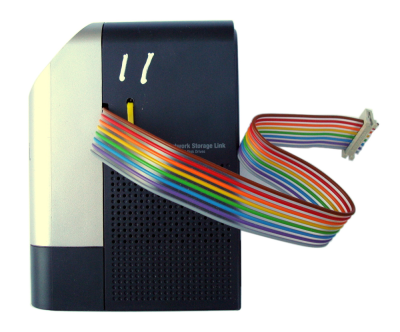
\includegraphics[height=2cm]{slug}  & Slug & 1 \\ \hline
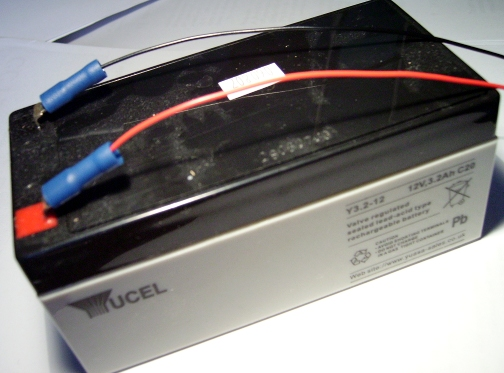
\includegraphics[height=2cm]{battery}  & 12V Sealed Lead Acid battery & 1 \\ \hline
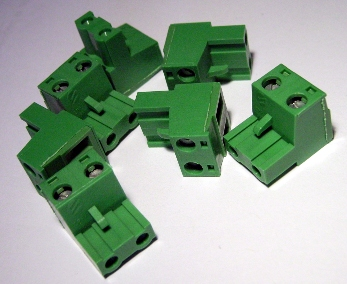
\includegraphics[height=2cm]{camcon}  & SR Connector & 4 \\ \hline
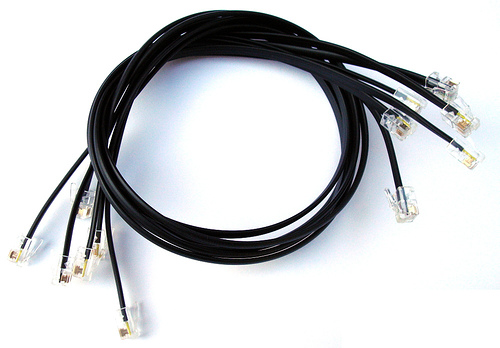
\includegraphics[height=2cm]{4p4c}  & RJ11 Cable & 5 \\ \hline
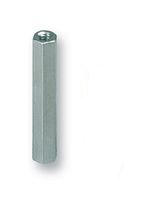
\includegraphics[height=2cm]{spacer}  & PCB Spacers & 17 \\ \hline
-  & USB Memory Stick & 2 \\ \hline
-  & Battery Charger & 1 \\ \hline
- & Web Camera & 1 \\ \hline
- & JointIO Board & 1 \\ \hline
- & Power Board & 1 \\ \hline
- & PWM Board & 1 \\ \hline
- & Motor Board & 1 \\ \hline
 - & USB Hub & 1 \\ \hline
\end{longtable}

\end {document}
